% What Context Compression Cannot Buy
% Draft 0.1 -- 2026-09-22
% pdflatex + bibtex + pdflatex x2. Standard packages only.
\documentclass[11pt]{article}
\usepackage[margin=1in]{geometry}
\usepackage{booktabs}
\usepackage{amsmath}
\usepackage{graphicx}
\usepackage{hyperref}
\usepackage{xcolor}
% Latin Modern is scalable; microtype's font expansion refuses to run on the
% default bitmap CM fonts.
\usepackage{lmodern}
\usepackage[T1]{fontenc}
\usepackage{microtype}
% \citet / \citep and the plainnat style both come from natbib; loaded before
% hyperref so the citation links are built correctly.
\usepackage{natbib}

\hypersetup{colorlinks=true, linkcolor=blue!50!black, citecolor=blue!50!black,
            urlcolor=blue!50!black}

% Draft markers -- every one of these must be gone before submission.
\newcommand{\TODO}[1]{\textcolor{red}{\textbf{[TODO: #1]}}}
\newcommand{\CHECK}[1]{\textcolor{orange}{[verify: #1]}}

\title{What Context Compression Cannot Buy:\\
       Diagnosing the Recall Ceiling with a Frozen Backbone}

\author{Xin Gao\\
  \texttt{hoshi@stu.xaut.edu.cn}}

\date{\today}

\begin{document}
\maketitle

\begin{abstract}
Compression of a transformer's KV cache is usually reported as one number: the
fraction of full-context quality retained. We ask what the missing fraction is
made of. Training only 3.67M memory-slot parameters with the backbone frozen,
we find that fraction is set by a single property of the task---how much of the
answer can be copied from the context rather than inferred.

Splitting predicted tokens on that property separates them sharply: tokens that
never appeared recover at $+202\%$, above the verbatim cache they replace, while
tokens seen exactly once reach $+45\%$. Posed as a task---recover a random
five-digit code hidden in the context---64 learned slots answer none of 150
trials and leave the model worse off than with no context at all, while the same
budget spent on verbatim entries answers $98\%$ when an oracle selects them and
$5\%$ when a drafted query does.

The same property predicts which methods win. Against three training-free
selection policies at an identical 576-entry budget, our hybrid recovers
$+89.5\%$ against a best baseline of $+55.8\%$ on held-out text---and on the
needle task the ranking inverts completely, ours placing last behind all three,
because its retrieval query is a guess and a random code cannot be guessed.
Across 0.6B to 14B, retrieval and abstraction are each flat while only their
combination moves, peaking at 1.7B--4B and falling below its starting value by
14B.

We also quantify two measurement hazards: fine-tuning the backbone improves the
no-context baseline by 0.58 nats, inflating every relative compression metric,
and pooling scale points measured under different quantisation and corpora
manufactured a clean monotone trend that a controlled sweep does not show.
\end{abstract}

\section{Introduction}

Work on shrinking the KV cache of a long-context transformer---by eviction, by
low-rank or low-bit approximation, by learned summarisation into a fixed budget
of slots---reports its result as a retention figure: this method keeps $x\%$ of
full-context quality at $y\times$ compression. The figure is useful for choosing
a method. It says nothing about the $1-x$.

This paper is about the $1-x$. We do not propose a compression method; several
of the components we use were introduced elsewhere and we cite them as such
(\S\ref{sec:related}). We use a deliberately minimal setup---a frozen backbone
with a few million trainable memory-slot parameters---as an instrument, and ask
two questions about where compressed context loses to verbatim context.

\paragraph{Contribution 1: the ceiling is made of precise recall
(\S\ref{sec:copyability}).}
We group the tokens being predicted by whether that token appeared anywhere in
the preceding context, i.e.\ by whether the answer was available to copy
(Table~\ref{tab:copyability}). The
groups behave qualitatively differently rather than by degree. On tokens that
never appeared, a 64-slot learned state recovers $+202\%$ of the gap between no
context and full context---it is more useful than the verbatim cache it replaces,
because it was optimised to predict the continuation whereas raw KV was not. On
tokens that appeared exactly once, the same state recovers $+45\%$. Since the
copyable group is $79.6\%$ of the suffix and carries $76.0\%$ of the gap, the
ceiling on abstractive compression is a property of the task, not a deficiency
of the compressor. We then state the same claim as a retrieval task
(\S\ref{sec:needle}), where the answer is a random code and abstraction is not
merely insufficient but actively harmful. The same axis turns out to predict
which \emph{retrieval} policies win: the ranking of four methods reverses
between the two regimes, ours included (\S\ref{sec:baselines}). To our knowledge this decomposition has not been reported for
compressed context; the nearest work stratifies tokens by $n$-gram novelty in
\emph{uncompressed} long-context models \citep{tokensbenefit}, or contrasts
topical against unexpected needles at the task level \citep{gistboundary}.

\paragraph{Contribution 2: retrieval and compression are separable and roughly
equal, and only their combination responds to scale
(\S\ref{sec:decomposition}, \S\ref{para:scale}).}
Pairing the abstract state with a small set of exactly-retrieved verbatim KV
entries is a natural architecture and has been proposed before
\citep{strongdrafts,specache}. What has not been measured, to our knowledge, is
the attribution: we fix the retrieved entries and swap only the state behind
them (absent / trained / randomly initialised), and independently fix the state
and swap only the anchor \emph{source} (a deployable query against an
answer-aware oracle). This closes a $2\times2$ design in which each factor's
contribution can be read holding the other fixed. Agent-memory systems have
compared ``read the summary'' against ``fetch the source''
\citep{justmem,infinimemory}, but with both the retrieval set and the summariser
varying together. The scale axis separates them a second time and by a different
mechanism: across four backbone sizes each component is flat on its own while the
hybrid is not, peaking in the middle of the range and ending below its starting
point (\S\ref{para:scale}). A single-resource account does not predict that.

\paragraph{Contribution 3 (a caveat, not a claim): two measurement hazards
(\S\ref{sec:hazards}).}
Relative compression metrics normalise by the distance between a no-context
lower bound and a full-context upper bound. If the backbone is fine-tuned during
compression training, the lower bound moves: we measure $0.58$ nats of
improvement on ``predict the continuation with no context at all,'' shrinking the
denominator by a third and inflating recovery from $+8\%$ to $+66\%$ on the
identical configuration. This is not a new observation so much as a
quantification of one: \citet{ccm} report the same phenomenon as a training
pathology (the model learns to answer without consulting its memory) and freeze
the LM in response, and \citet{simplecc} adopt an almost identical normalisation
to control for questions answerable without context. Our contribution is to
frame it as an \emph{evaluation} confound with a measured magnitude, and to note
the boundary: it affects relative metrics only, not absolute task accuracy.
Second, we report seed variance, which is rarely reported in this literature and
is largest exactly where it matters most. We also give two worked examples of
what skipping this costs, both from our own earlier drafts of the scale
comparison: mismatched prediction lengths put the gap at 0.492 against 0.822
nats and made the recovery figures incomparable, and pooling points measured
under different quantisation and corpora produced a clean monotone trend that
the controlled sweep does not show (\S\ref{para:scale}).

\section{Setup}
\label{sec:setup}

\paragraph{Compressor.}
A context window of $n$ tokens is consumed in segments. Each segment is encoded
with the frozen backbone and reduced to $k$ learned memory slots, which are
prepended to the next segment's attention as synthetic KV entries. The only
trainable parameters are the slot embeddings ($0.03$M) and, in the \emph{deep}
variant, a per-layer additive bias applied at memory positions only
($3.67$M, in the manner of prefix tuning \citep{ptuningv2}). Because attention is
causal and the bias is restricted to memory positions, the backbone's behaviour
on real tokens is bit-identical to the unmodified model.

\paragraph{Metric.}
For a held-out suffix we measure mean token cross-entropy under three
conditions: \textsc{upper} (the full verbatim KV cache of all $n$ preceding
tokens), \textsc{lower} (no context at all), and the condition under test. We
report
\begin{equation}
\text{recovery} = \frac{\textsc{lower} - \text{test}}{\textsc{lower} - \textsc{upper}},
\label{eq:recovery}
\end{equation}
in nats. $1.0$ means indistinguishable from the full cache and $0$ means the
context was worthless. \textbf{Values above $1.0$ are attainable and are not an
error}: the learned slots are trained to predict the next segment, whereas the
verbatim cache is simply what the model happened to write down, so a compressed
state can be more useful than the text it summarises. We call
$\textsc{lower}-\textsc{upper}$ the \emph{gap}, and note that it is a property of
the corpus rather than of the method: it is $1.269$ nats on real dialogue and
$0.286$ nats on Project Gutenberg prose, meaning long context is worth little on
coherent narrative to begin with (\S\ref{sec:limitations}).

\paragraph{Anchors.}
In the hybrid conditions, a budget of $a$ verbatim KV entries (``anchors'') is
selected from the offloaded full cache and paged back in alongside the $k$ slots.
Selection policies are compared in \S\ref{sec:decomposition}. Two details are
load-bearing and easy to get wrong. First, any scheme that retains only part of
the cache must pin the first few positions as an \emph{attention sink}
\citep{streamingllm}; without it recovery collapses to $-400\%$. Second,
positions must accumulate across segments rather than restart, which is worth
4 points.

\paragraph{Scale and cost.}
Qwen3-0.6B \citep{qwen3} for every measurement, with the hybrid architecture
checked against 1.7B (\S\ref{sec:levers}); windows of 4096 tokens in
\S\ref{sec:copyability} and 8192 in \S\ref{sec:decomposition}, stated per table
because the two are not comparable. Everything ran on a single RTX 4060 Laptop
(8\,GB); training one memory module takes roughly 12 minutes, and no cloud
compute was used for any number in this paper.

\section{The ceiling is made of precise recall}
\label{sec:copyability}

Two levers that should raise a compressor's ceiling do not
(\S\ref{sec:levers}): more training and more slots. At a fixed backbone, then,
the residual is not something the compressor is failing to try hard enough at.
The candidate is precise recall---the identifier introduced 2000 tokens ago, the
number, the proper noun. Verbatim KV can be copied from. A summary cannot
reconstruct a string it did not store. Scale does move the level
(\S\ref{para:scale}), and we return at the end of this section to what it does
and does not change.

We test this by partitioning the predicted suffix. For each target token we ask
whether that token appears anywhere in the preceding context, and compute
per-token cross-entropy within each group under all three conditions. Only the
abstract state is provided---no anchors---so the comparison isolates what
abstraction alone can serve.

\begin{table}[ht]
\centering
\small
\begin{tabular}{lrrrrr}
\toprule
target token & share & \textsc{lower} & \textsc{upper} & gap (nats) & recovery \\
\midrule
never appeared      & 20.4\% & 5.731 & 5.518 & $\mathbf{0.213}$ & $+202\%$ \\
appeared            & 79.6\% & 3.542 & 2.401 & $\mathbf{1.141}$ & $+58\%$ \\
\quad exactly once  &  9.6\% & 5.190 & 4.014 & 1.176 & $+45\%$ \\
\quad 2--5 times    & 19.4\% & 4.539 & 3.045 & 1.494 & $+48\%$ \\
\quad 6+ times      & 50.6\% & 2.848 & 1.849 & 0.999 & $+67\%$ \\
\midrule
all                 & 100\%  & 3.989 & 3.038 & 0.951 & $+65\%$ \\
\bottomrule
\end{tabular}
\caption{Cross-entropy by token copyability, abstract state only (64 slots,
8 hops over 4096 tokens), mean of three independently trained modules.
\textsc{lower} is no context, \textsc{upper} the full verbatim cache. Seed
spread is 3.0--4.3 points on the large groups but 9.1 on ``exactly once''
($n{=}1176$) and 11.3 on ``never appeared'', where the small gap in the
denominator amplifies it---see the caution below.}
\label{tab:copyability}
\end{table}

\paragraph{Read the gap column first.}
The cleanest statement here does not involve our metric at all. Having the entire
verbatim context is worth $1.141$ nats on tokens that appeared in it and $0.213$
nats on tokens that did not. Long context earns most of its value on material
that can be copied: the copyable group is $79.6\%$ of the suffix and carries
$76.0\%$ of the total gap, a figure identical across all three seeds because it
depends only on the corpus and not on the module. Whatever a compressor does,
this is the shape of what it is compressing.

\paragraph{Recovery, with a caution about the denominator.}
On tokens that never appeared, the 64-slot state recovers $+202\%$---substantially
more useful than the verbatim cache it replaces, because it was trained to
predict the continuation whereas the cache is merely what the model wrote down.
On tokens that appeared exactly once it recovers $+45\%$, and recovery rises
monotonically with how often the token was seen ($+45 \to +48 \to +67$). The
caution: those extreme groups also carry the largest seed spread, and not by
accident. Recovery divides by the gap; the never-appeared gap is $0.213$ nats;
dividing by a small number magnifies everything, including noise. The ordering is
robust---$+202$ against $+58$ is a separation of 144 points against spreads of 11
and 4---but the value $202$ itself is not stable to three significant figures,
and we would not report it without the gap column beside it. This is a general
hazard when a relative compression metric is evaluated on subsets, and a reason
to prefer absolute nats when slicing.

\paragraph{The ordering is a property of the task; the levels are not.}
Repeating the split at 0.6B and 4B separates what is fixed from what is not.

\begin{table}[ht]
\centering
\small
\begin{tabular}{lrrrrr}
\toprule
 & once & 2--5 & 6+ & never & all \\
\midrule
0.6B & $+30.9$ & $+40.1$ & $+60.1$ & $+126.7$ & $+53.6$ \\
4B   & $+56.6$ & $+56.7$ & $+71.0$ & $+165.2$ & $+72.7$ \\
\midrule
change & $\mathbf{+25.7}$ & $+16.6$ & $\mathbf{+10.9}$ & $+38.5$ & $+19.1$ \\
\bottomrule
\end{tabular}
\caption{The same partition at two scales, single seed each. Two mismatches make
the absolute values here lower than Table~\ref{tab:copyability} and not
comparable to it: these modules were trained at the shorter prediction length
and evaluated over a full segment, and the 4B backbone is NF4-quantised while
0.6B is bf16. Only the pattern across columns should be read. 1.7B is omitted
because that particular checkpoint diverged under recursion
(\S\ref{sec:limitations}).}
\label{tab:copyscale}
\end{table}

Which tokens are hard does not change---the ordering holds at both scales, and
tokens seen once remain the worst-served group by a wide margin. How hard they
are does change, and in the direction we did not predict: the hardest column
improves most ($+25.7$) and the easiest improves least ($+10.9$). So the ceiling
is not a fixed property of abstractive compression. It is a property of what a
\emph{given} backbone can compress, and a larger one recovers a substantial part
of what the smaller one loses on precisely the tokens we called incompressible.
We therefore state the finding as the ordering rather than the level, and note
that an extrapolation to ``a large enough model would not need exact recall at
all'' is not supported by two points.

\paragraph{What follows.}
Two readings. First, abstraction is not a degraded copy of verbatim context but a
different thing---better on some tokens, much worse on others. Aggregate recovery
figures approaching $100\%$ should therefore not be read as ``nearly as good as
having the text,'' since they average over groups that behave in opposite
directions. Second, the practical one: at a fixed backbone the residual lives in
copyable tokens, and the way to buy it back is not a larger abstraction
budget---\S\ref{sec:levers} shows doubling it buys $0.6$ points---but a small
number of \emph{exact} entries. \S\ref{sec:decomposition} measures what that
buys.

\subsection{The same claim, stated as a task}
\label{sec:needle}

Everything above is perplexity on held-out text, which is the form of evidence a
reader has least reason to trust. The claim it supports---that what compression
cannot buy is precise recall---can be stated as a task instead. We hide a
uniformly random five-digit code in the context (``the secret code for
warehouse 7 is 48213''), place the question at the end, and ask for the digits
back. Copyability here is total rather than statistical: the code is drawn at
generation time, so no prior over language helps, and a memory that did not
store the digits cannot produce them.

\begin{table}[ht]
\centering
\small
\begin{tabular}{lrrr}
\toprule
memory available at question time & recovery & exact match & gap closed \\
\midrule
full verbatim cache (4096 tokens)      & $+100\%$  & $\mathbf{100\%}$ & --- \\
no context                             & $0\%$     & $0\%$   & --- \\
\midrule
64 abstract slots                      & $\mathbf{-28.6\%}$ & $\mathbf{0\%}$ & none \\
512 anchors, deployable retrieval      & $+14.9\%$ & $5\%$   & partial \\
512 anchors $+$ 64 slots               & $+14.3\%$ & $3\%$   & partial \\
512 anchors, oracle retrieval          & $+94.4\%$ & $\mathbf{98\%}$ & nearly all \\
\bottomrule
\end{tabular}
\caption{Needle retrieval, 4096-token contexts, 3 seeds $\times$ 5 needle
depths $\times$ 10 samples $=$ 150 trials per condition. Recovery is over the
answer tokens only. The gap between no context and full context is $2.52$ nats
here against $0.95$ on dialogue, which is what a task built entirely out of
uncopyable answers looks like.}
\label{tab:needle}
\end{table}

Three readings, in increasing order of what they cost us.

\paragraph{The abstract state does not merely fail; it is worse than nothing.}
Sixty-four learned slots that recover most of the loss on ordinary text answer
zero of 150 needles, and leave the model \emph{worse off} than having no context
at all ($-28.6\%$, consistent across seeds). The slots occupy attention while
carrying nothing relevant to the question. This is \S\ref{sec:copyability}'s
``exactly once'' column taken to its limit, and it is the cleanest statement we
can make of what abstraction cannot do.

\paragraph{Adding the state to retrieval makes things slightly worse, not
better.} On dialogue the same state is worth $+44$ points behind the same
anchors (\S\ref{sec:decomposition}); here it costs 2 points of exact match. The
value of a compressed memory is not a property of the compressor at all: it is
set by how much of the answer the task allows to be copied.

\paragraph{Selection is the whole task, in a way it is not on text.}
Identical budget---512 verbatim entries---answers $98\%$ of needles when chosen
by an oracle and $5\%$ when chosen by attention over the question. Broken down
by needle depth, the deployable policy pages in the needle at all for only two
of the five depths (0.3 and 0.9, in all three seeds), and at depth 0.9 it
retrieves the needle and still answers nothing: the several hundred irrelevant
entries paged in alongside it are enough to bury the one that mattered. Missing
the needle and drowning it are separate failures, and both are selection
problems.

This is the counterpart to the diffuseness we report in
\S\ref{sec:decomposition}, where a policy agreeing with the oracle on $8.5\%$ of
positions still captured three quarters of the available value. Both are true,
of different tasks: value is spread thinly over natural text and concentrated in
a single span here, and a retrieval policy that is adequate under the first
regime can be useless under the second. We would expect any evaluation of
KV-cache retrieval to move sharply depending on which regime its benchmark
samples, and \S\ref{sec:copyability}'s decomposition is a way to say in advance
which one a corpus is.

\section{Separating retrieval from compression}
\label{sec:decomposition}

The architecture under test pairs $k=64$ abstract slots with $a=512$ verbatim KV
entries paged back from an offloaded full cache: a 576-entry budget against 8192
tokens, $14{:}1$. Both halves are prior art (\S\ref{sec:related}). The question
here is only how the credit divides.

We vary two factors independently. \emph{Anchor source} is either the deployable
policy---a short speculative draft of the continuation, generated from the state
and the attention sink alone, used as the retrieval query \citep{specache}---or an
\emph{oracle} that is allowed to see the tokens being predicted and selects the
entries that actually help. \emph{State} is either absent, or the rolling state
that has compressed all 8192 preceding tokens, or a state that compresses only
the most recent segment (\S\ref{sec:levers} explains why the latter is better).
All six cells use the identical retrieved entries within a row and the identical
state within a column, so each difference is attributable.

\begin{table}[ht]
\centering
\begin{tabular}{lccc}
\toprule
anchor source & no state & rolling state & last-segment state \\
\midrule
speculative (deployable) & $+31.4$ & $+71.9$ & $+75.4$ \\
oracle (answer-aware)    & $+58.1$ & $+96.1$ & $\mathbf{+98.0}$ \\
\bottomrule
\end{tabular}
\caption{Recovery at a 576-entry budget over 8192 tokens ($14{:}1$), mean of
three independently trained memory modules. Seed spread is 1.6--2.3 points in
every cell; the no-state oracle cell is identical across seeds to four decimal
places, as it must be, since neither the oracle's selection nor the empty state
depends on the trained module---a consistency check on the measurement rather
than a result.}
\label{tab:twobytwo}
\end{table}

\paragraph{The two contributions are roughly equal and close to additive.}
Reading along the first row of Table~\ref{tab:twobytwo}, adding the abstract state behind a fixed set of
retrieved entries is worth $+44.0$ points; along the second row, behind the
oracle's entries, $+39.9$. Reading down the last column, replacing the deployable
retrieval with perfect selection is worth $+22.5$ points; down the first column,
$+26.7$. Each factor is therefore worth slightly less when the other is already
strong---the two memories are mildly redundant---but the interaction is small
relative to either main effect: starting from retrieval alone at $+31.4$ and
adding both main effects predicts $+102.1$ against an observed $+98.0$, an
interaction of $-4.1$ points. Compression and retrieval are close to separate
resources, and neither dominates. Both main effects are an order of magnitude
larger than the seed spread, which is what licenses reading them at all.

\paragraph{The budget is not the binding constraint; selection is.}
The best cell reaches $+98.0\%$ using $576$ of $8192$ entries---$7\%$ of the
cache---so essentially everything the full cache provides is reachable at this
budget \emph{if the right entries are chosen}. The deployable policy reaches
$+75.4\%$. The remaining $22.5$ points are a selection problem, not a capacity or
a compression problem, which is worth knowing before spending effort on better
compressors.

A detail sharpens this. The deployable policy's choices overlap the oracle's on
only $8.5\%$ of positions, yet it captures roughly three quarters of the
available value. The value is therefore diffuse: many different subsets of the
cache are nearly as good, and there is no small set of critical entries that a
retrieval policy must find. That is encouraging for cheap heuristics and
discouraging for the idea that a sharper query is the main thing missing.

\paragraph{Randomly initialised slots are worse than no slots at all.}
Substituting untrained slots for the trained state, holding the retrieved entries
fixed, does not merely remove the state's contribution---it lands far below the
no-state condition, between $-45\%$ and $-97\%$ across runs against $+31.4\%$ with
no state at all. (We report a range rather than a mean: the slots are re-drawn
per window and the draw is not seeded, so this condition is the one place where
run-to-run variation is expected and large. Its sign and magnitude are stable;
its exact value is not.) Synthetic
KV entries that lie outside the distribution the backbone expects actively
corrupt attention over the real entries beside them. Two consequences: the
$+44.0$ points above are a property of the trained state and not of merely
occupying positions; and any scheme that writes fabricated entries into a frozen
model's cache is working inside a narrow tolerance. Relatedly, every partial-cache
condition here must pin the first few positions as an attention sink, without
which recovery falls to roughly $-400\%$ \citep{streamingllm}.

\subsection{Against training-free selection at the same budget}
\label{sec:baselines}

The decomposition above says the learned state is worth $+44$ points behind
fixed anchors. A reader is entitled to a blunter question: at the same memory,
does any of this beat simply keeping the right 576 entries? Three well-known
policies answer that without training anything.

\begin{table}[ht]
\centering
\small
\begin{tabular}{lrrr}
\toprule
policy at 576 entries & recovery & seed spread & sink kept \\
\midrule
StreamingLLM \citep{streamingllm} & $+55.8\%$ & --- & 4/4 \\
SnapKV \citep{snapkv}             & $+53.1\%$ & --- & 4/4 \\
H2O \citep{h2o}                   & $+50.5\%$ & --- & 4/4 \\
\midrule
ours: 512 speculative anchors $+$ 64 slots & $\mathbf{+89.5\%}$ & $1.7$ & 4/4 \\
ours, with oracle anchors                  & $+103.2\%$ & $0.6$ & --- \\
\bottomrule
\end{tabular}
\caption{Identical budget, 4096-token contexts, 12 windows. The three baselines
are deterministic given the model, so their figures are identical across the
three seeds; ours varies with the trained module. ``sink kept'' is how many of
the first four positions each policy selected \emph{on its own}---we did not
force a sink on H2O or SnapKV, and all three mechanisms find the opening
anyway.}
\label{tab:baselines}
\end{table}

\paragraph{What this does and does not establish.}
The gap is large---33.7 points over the best baseline---but the comparison is
not like-for-like and we would rather say so than let a reader discover it. Our
method trains 3.67M parameters for roughly 12 minutes on one 8\,GB card; the
baselines train nothing. What the table supports is that \emph{at a fixed memory
budget} a small learned component buys far more than reallocating the same
entries, not that selection policies are poorly designed. Their design target is
different: they run without a training step and without a corpus, which is
exactly what makes them deployable where our module is not
(\S\ref{sec:limitations} states the domain-specificity that follows from
training on a corpus).

We implemented all three from the mechanisms their papers describe rather than
porting reference code, because the reference implementations are bound to
particular serving stacks and moving them here would make the comparison about
implementations. Attention scores are computed identically for every policy,
including ours---the last block's query projection against the cached keys---so
no policy is advantaged by a different notion of ``important''.

\paragraph{The simplest baseline is the strongest one.}
StreamingLLM keeps the sink and the most recent window and consults no attention
statistic at all. It beats both policies that do ($+55.8$ against $+53.1$ and
$+50.5$). That ordering is the same phenomenon as
\S\ref{sec:decomposition}'s diffuseness: when the value of the context is spread
thinly, a policy that simply keeps the nearest tokens captures much of it, and
the extra machinery of scoring every position earns little. \S\ref{sec:needle}
shows the regime where this reverses---there, recency is worthless because the
needle is not recent, and selection is everything.

\paragraph{On the other regime, the ordering inverts and our method comes last.}
Running the same four policies on the needle task of \S\ref{sec:needle} reverses
the table completely (Figure~\ref{fig:inversion}).

\begin{table}[ht]
\centering
\small
\begin{tabular}{lrrrr}
\toprule
 & \multicolumn{2}{c}{natural text} & \multicolumn{2}{c}{needle} \\
\cmidrule(lr){2-3}\cmidrule(lr){4-5}
policy & recovery & rank & exact match & rank \\
\midrule
ours (speculative $+$ slots) & $\mathbf{+89.5\%}$ & 1 & $3\%$ & \textbf{4} \\
StreamingLLM                 & $+55.8\%$ & 2 & $20\%$ & 2 \\
SnapKV                       & $+53.1\%$ & 3 & $\mathbf{24\%}$ & \textbf{1} \\
H2O                          & $+50.5\%$ & 4 & $5\%$ & 3 \\
\midrule
oracle anchors               & $+103.2\%$ & --- & $98\%$ & --- \\
\bottomrule
\end{tabular}
\caption{The same policies at the same budget on two tasks. Needle figures are
3 seeds $\times$ 50 trials; the seed spread on exact match is 0--8 points, well
below the differences between policies.}
\label{tab:inversion}
\end{table}

\begin{figure}[ht]
\centering
\includegraphics{fig_inversion.pdf}
\caption{Rank of each policy on the two tasks, at the same 576-entry budget
(values in parentheses; the two tasks use different metrics, so only the
ordering is comparable). Our method is first on held-out text and last on the
needle, and the three training-free policies reorder among themselves as well.}
\label{fig:inversion}
\end{figure}

We report this because it is the sharpest test the paper contains and it goes
against us. Our method is first by 34 points on held-out text and last on the
needle, below every training-free policy it beat.

The mechanism is not mysterious, and it is the retrieval query rather than the
compressor. SnapKV scores context positions by the attention of a window at the
\emph{end of the prompt}---which on this task is the question, and the question
names what is wanted. Our policy drafts a continuation and retrieves what the
draft attends to (\S\ref{sec:decomposition}), which works when the continuation
is guessable and fails exactly when it is not. A uniformly random five-digit
code is the worst case for a method whose query is a guess. StreamingLLM lands
in between for a third reason entirely: it holds the most recent window, so it
succeeds on the one depth in five where the needle happens to be recent, which
is precisely the $20\%$ observed.

So the axis of \S\ref{sec:copyability} predicts more than where the compression
ceiling sits. It also predicts which retrieval signal is available: where
continuations are inferable, a drafted query is informative and beats attention
statistics; where the answer is arbitrary, only a query derived from the actual
request helps, and a compressed summary alongside it is dead weight
(\S\ref{sec:needle}). A method should be reported against the regime it targets,
and ours targets the first. We would not deploy it as written for
needle-retrieval, and \S\ref{tab:inversion} is the reason.

\section{What moves the ceiling, and what does not}
\label{sec:levers}

\begin{table}[ht]
\centering
\small
\begin{tabular}{llcc}
\toprule
lever & range & deployable & retrieval only \\
\midrule
training on the recursion & init $\to$ 600 steps & $+59.9 \to +58.6$ & --- \\
abstract slot budget      & 64 $\to$ 128 slots   & $+67.0 \to +67.6$ & --- \\
anchor budget             & 512 $\to$ 1024 entries & $+87.8 \to +96.6$ & --- \\
\midrule
backbone scale & 0.6B $\to$ 14B & non-monotone, peak $\mathbf{+90.2}$ & flat \\
\bottomrule
\end{tabular}
\caption{Training and abstraction budget do not move the ceiling; anchor budget
does, by spending memory on verbatim entries. Scale moves it non-monotonically,
rising to a peak at 1.7B--4B and then declining over 8B and 14B to below its
starting value, while retrieval on its own stays within 9 points across a
23-fold parameter range; Table~\ref{tab:scale} gives that sweep in full. The first three rows are earlier experiments at their own
settings and are not comparable to the fourth.}
\label{tab:levers}
\end{table}

\paragraph{Training the recursion trades near for far.}
Six hundred steps of training dedicated to the recursion itself leave the 8-hop
figure where it started ($+59.9 \to +58.6$) while the 1-hop figure falls from
$+128.8$ to $+98.8$. The module does not become better at carrying information
across many hops; it becomes worse at the single hop in exchange for nothing. We
read this as the loss occurring at each re-encoding rather than at the point of
storage. Doubling the slot budget likewise buys $0.6$ points, so neither
capacity nor training is the binding constraint.

\paragraph{Scale moves the combination, not the components.}
\label{para:scale}
Sweeping 0.6B to 14B under matched conditions separates three quantities that a
pooled comparison would confound.

\begin{table}[ht]
\centering
\small
\begin{tabular}{lrrrrrr}
\toprule
 & 0.6B & 1.7B & 4B & 8B & 14B & 8B\,(lr 2e-3) \\
\midrule
512 anchors alone            & $+21.0$ & $+26.9$ & $+26.0$ & $+26.9$ & $+30.1$ & $+26.9$ \\
576 slots, all abstraction   & $+59.6$ & $+53.3$ & $+59.6$ & $+59.3$ & $+53.9$ & $+57.7$ \\
\midrule
\textbf{512 anchors $+$ 64 slots} & $+82.6$ & $\mathbf{+90.2}$
  & $\mathbf{+90.1}$ & $+83.3$ & $+75.9$ & $+82.7$ \\
\quad gain over better component & $+23.0$ & $+36.9$ & $+30.5$ & $+24.0$ & $+22.0$ & $+23.0$ \\
\midrule
\quad same, absolute (nats)  & $0.807$ & $0.866$ & $\mathbf{0.880}$ & $0.807$ & $0.779$ & $0.802$ \\
\quad gap (denominator)      & $0.977$ & $0.960$ & $0.977$ & $0.969$ & $1.026$ & $0.969$ \\
\quad memory params          & 3.7M & 7.3M & 11.8M & 18.9M & 26.2M & 18.9M \\
\bottomrule
\end{tabular}
\caption{Identical budget (576 entries) spent three ways, at five scales. Each
column is one training run; the last repeats 8B at a lower learning rate. The
components are flat and the combination is not. Because 14B's gap is $0.066$
nats wider than the others', the row above it gives the same quantity in
absolute nats---both readings give the same shape, so it is not an artefact of
the normalisation.}
\label{tab:scale}
\end{table}

\begin{figure}[ht]
\centering
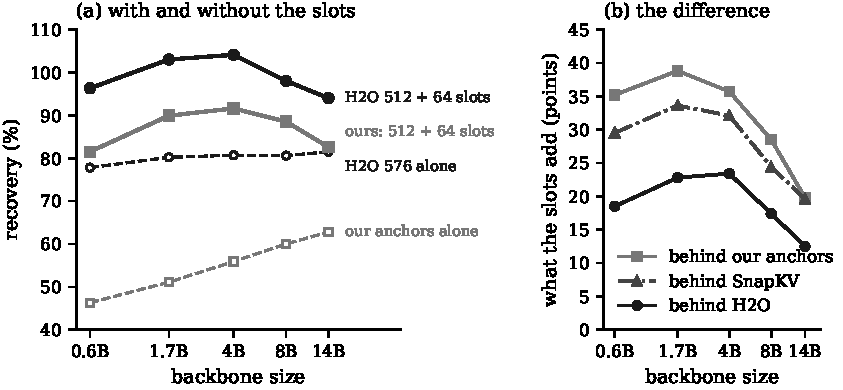
\includegraphics{fig_scale.pdf}
\caption{The same numbers as Table~\ref{tab:scale}. Each component is flat
across a 23-fold range of parameters; only their combination moves, and it ends
below where it began. The dotted line marks the 0.6B value.}
\label{fig:scale}
\end{figure}

Figure~\ref{fig:scale} shows the shape. Retrieval alone is flat: 512 verbatim
entries are worth $+21$ to $+30$ across a 23-fold range of parameters. Abstraction alone is flat: the same budget spent
entirely on learned slots recovers $+53$ to $+60$ everywhere. Only the
combination moves, and it moves non-monotonically---up 7.6 points from 0.6B to
1.7B, flat to 4B, then down at 8B and further at 14B, finishing 6.7 points
\emph{below} where 0.6B started. The peak is in the middle of the range and the
decline past it is monotone over two further points.

The 8B figure is not an artefact of a bad run. Its first training used the
learning rate tuned at 0.6B, whose curve peaked at $+92.3\%$ around step 500 and
stepped down to $+86\%$ by step 800---the signature of too large a step size,
and the checkpoint we must use is the final one. Retraining at $2.5\times$ lower
learning rate produced a healthier curve and a training figure 3.3 points
better, and moved the deployable hybrid by $-0.6$ points. Two runs differing in
learning rate and seed agree to within a point, so the drop is a property of the
scale point under this architecture.

What scales, then, is neither memory on its own. It is how well the two work
together: the gain of the hybrid over the better of its two components peaks at
1.7B and falls steadily thereafter. We do not have a mechanism, and the obvious
candidate does not survive contact with the data. The memory module's parameter
count grows with the backbone (3.7M, 7.3M, 11.8M, 18.9M, 26.2M) against a fixed
training budget, so under-training would predict the \emph{smallest} module to
do best---but 0.6B is not the peak either, and the maximum sits at 7--12M
parameters with both ends lower. Something about the middle of this range suits
a 64-slot summary paired with exact anchors, and five points do not say what.

One further observation, offered as a lead rather than an explanation:
randomly initialised slots are catastrophic at 0.6B ($-35.6\%$) and nearly
harmless at 14B ($+47.3\%$, against $+49.1\%$ for no slots at all). Larger
backbones tolerate arbitrary synthetic KV entries that smaller ones cannot read.
Whatever makes a large model forgiving of noise in its cache may also make it
indifferent to the structure a trained compressor puts there.

\paragraph{Reading this result carefully.}
Two cautions, because the shape of this curve invites over-reading. First, each
scale point is a single training run apart from 8B; the seed spread measured at
0.6B elsewhere in this paper is 1.0--1.4 points on these conditions, which is
well below the 7-point swings here but is an extrapolation to the larger points.
Second, and more important for anyone extending this: we obtained a clean
monotone increase from an earlier, pooled version of this comparison, in which
the 4B point came from a different machine, a different quantisation and a
different corpus than the others. Each individual correction was small---1.2
points for NF4, 0.3 for the corpus---and together they manufactured a trend that
the controlled sweep does not show. Small, individually defensible corrections
compose into artefacts.

\paragraph{The effective window is about one segment.}
A rolling state that has passed over all 8192 tokens recovers $+61.5\%$;
compressing \emph{only the most recent 512} recovers $+65.6\%$. Carrying the
state forward therefore dilutes rather than accumulates, and the distant past is
better served by anchors than by a longer chain of compression. Recurrent
compressive memories are known to concentrate on the recent past
\citep{compressive,lcirc}; the contribution here is that on this task the rolling
variant is not merely no better but worse than not rolling at all, which changes
what one should build.

\section{Two measurement hazards}
\label{sec:hazards}

\subsection{Fine-tuning the backbone deflates the denominator}

\begin{table}[ht]
\centering
\begin{tabular}{lcccc}
\toprule
 & \textsc{upper} & \textsc{lower} & gap & recovery \\
\midrule
backbone frozen & 3.459 & 3.951 & 0.492 & $\mathbf{+66\%}$ \\
LoRA enabled    & 3.037 & $\mathbf{3.370}$ & $\mathbf{0.332}$ & $+8\%$ \\
\bottomrule
\end{tabular}
\caption{Identical learning rate, identical step count; the only difference is
whether the backbone may adapt. The adapter improves ``predict the continuation
from nothing'' by 0.58 nats, removing a third of the denominator in
Eq.~\ref{eq:recovery}.}
\label{tab:lora}
\end{table}

The adapter is not learning to compress. It is doing language-model fine-tuning
on the evaluation distribution, and one side effect is that the task gets
easier. Note the direction of the trap: here it made the frozen number look
better, because the same slots were measured against an undeflated denominator.
In general the sign depends on which configuration is being promoted, which is
precisely why the confound is worth naming.

\paragraph{Scope.} This affects relative metrics of the form
Eq.~\ref{eq:recovery} only. Work reporting absolute downstream accuracy is
unaffected, and work that fine-tunes both a compressor and a reader for
deployment is doing something legitimate that this critique does not touch. See
\S\ref{sec:related} for the closest prior statements.

\subsection{Variance is largest where the headline is}

\begin{table}[ht]
\centering
\begin{tabular}{lccccr}
\toprule
configuration & seed 0 & seed 1 & seed 2 & & spread \\
\midrule
16 slots ($32{:}1$) & $+15$ & $+41$ & $+66$ & & \textbf{51 points} \\
32 slots ($16{:}1$) & $+105$ & $+66$ & $+103$ & & \textbf{39 points} \\
72 slots & $+114$ & $+109$ & $+111$ & & 5 points \\
128 slots & $+115$ & $+111$ & $+112$ & & 4 points \\
\midrule
hybrid, six conditions (\S\ref{sec:decomposition}) & & & & & 1.6--2.3 points \\
\bottomrule
\end{tabular}
\caption{Identical data and hyperparameters; only the random seed differs. The
first four rows are single-hop recovery measured during training, which is why
they exceed $100\%$ and are not comparable to the multi-hop figures elsewhere;
what matters is the spread down each row. The last row covers the six cells of
Table~\ref{tab:twobytwo}, excluding the randomly initialised state, whose slots
are re-drawn per window and unseeded by construction.}
\label{tab:variance}
\end{table}

The compression ratios that are most attractive to report are the ones whose
results are least reproducible. We found this the hard way: a checkpoint was
lost and retrained under identical settings, and the 16-slot figure moved from
$+83\%$ to $+38\%$. Any claim in this area resting on a few points---including
several we had provisionally drawn about scale---requires its own spread before
it means anything. We recommend reporting seed spread at the highest compression
ratio claimed, and we note that the hybrid architecture is not merely better on
average but an order of magnitude more stable, which may be the more important
property.

\section{Related work}
\label{sec:related}

Our instrument is assembled from published components; what follows separates
what we borrowed from what we are claiming.

\paragraph{Discarding or approximating real cache entries.}
One family keeps the cache made of real entries and decides which to drop.
\citet{h2o} retain a recent window plus persistent heavy hitters identified by
accumulated attention; \citet{snapkv} select using an observation window at the
end of the prompt; \citet{pyramidkv} allocate unequal budgets across depth.
\citet{streamingllm} show that the first few positions act as an attention sink
whose removal is catastrophic---a result we depend on operationally, since every
partial-cache condition in this paper would otherwise collapse.
\citet{kivi} approximate rather than evict, quantising the cache to two bits.
\citet{quest} and \citet{infllm} keep the full cache but attend sparsely, scoring
blocks or representative tokens to decide what to load. These methods never
fabricate entries, so the distribution constraint we report in
\S\ref{sec:decomposition}---that untrained synthetic slots are worse than no
slots---does not arise for them. We do not benchmark against this family
(\S\ref{sec:limitations}).

\paragraph{Learning to compress context into slots.}
The second family replaces spans of context with a small number of learned
vectors: gist tokens \citep{gist}, autoencoding into memory slots \citep{icae},
summary vectors trained by continued adaptation \citep{autocompressor}, and
aggressive prompt compression \citep{500x}. Recurrent variants compress
repeatedly as the sequence advances \citep{compressive,rmt,lcirc}. Our compressor
is a minimal member of this family---learned slot embeddings plus a per-layer
bias at memory positions in the manner of prefix tuning \citep{ptuningv2}---and we
make no claim for it. We hold the backbone frozen throughout, which within this
family is closest to \citet{icae}, \citet{arcencoder} and \citet{500x}.

\paragraph{Pairing compressed memory with exact entries.}
The hybrid we measure has been proposed. \citet{strongdrafts} combine compressed
distant slots with exact recent entries for speculative decoding, discarding the
distant verbatim cache rather than retrieving it. \citet{specache} keep verbatim
KV on the CPU and prefetch it by predicting what the next step will attend to,
which is the speculative-retrieval mechanism we use as our deployable policy. At
the agent-memory level, \citet{justmem} and \citet{infinimemory} both contrast
reading a compressed representation against fetching the source, and both find
neither alone suffices---consistent with our decomposition, though at the level
of task accuracy with retrieval set and summariser varying together, rather than
holding one fixed to attribute the difference. We treat all four as prior art for
the architecture and confine our claims to the attribution.

\paragraph{Whether to freeze the reader.}
Freezing is usually motivated by plug-and-play reuse or by preserving abilities
outside the compression task \citep{icae,arcencoder,500x}; \citet{cocom} argue the
opposite for retrieval-augmented generation, holding that a frozen decoder cannot
make good use of compressed context, and \citet{spkv} continue pretraining the
model jointly with their utility predictor. Closest to \S\ref{sec:hazards},
\citet{ccm} report that naively fine-tuning the whole model during compression
training lets it answer without consulting the memory at all---their no-context
training loss falls from 2.69 to 1.84 while test loss stays at 2.59---and freeze
the LM in response. They frame this as overfitting on inputs, i.e.\ a training
pathology. \citet{simplecc} adopt a normalisation nearly identical to
Eq.~\ref{eq:recovery} in order to discount questions answerable without context,
but fine-tune adapters on both sides and present the correction as a property of
the question set. Our addition is narrow: the same effect read as an
\emph{evaluation} confound, with a magnitude attached (0.58 nats, a third of the
denominator) and a stated scope. We do not claim the principle is new.

\paragraph{Compressibility depends on the task.}
That compression costs vary sharply across task types is established
\citep{kvbench,shotkv}. Our dialogue-versus-prose gap figures (1.269 against 0.286
nats) are reported in that spirit---as a caution about which corpora can support
this measurement at all---and not as a finding.

\paragraph{Per-token analyses of long context.}
Nearest to \S\ref{sec:copyability}, \citet{tokensbenefit} stratify token-level
perplexity by how often an $n$-gram occurs in the added context and find that
newly appearing material correlates with the benefit from a longer window, but
they study \emph{uncompressed} long-context models, so the question of what
compression specifically destroys does not arise. \citet{gistboundary} analyse
gist-based compression at finer grain than task accuracy and find unexpected
information is lost preferentially---topically relevant word needles at 50.7
against surprising ones at 35.8 under $8\times$ compression---which points the
same direction as our result while grouping by a needle's relation to the topic
rather than by whether the target token was copyable. To our knowledge the
grouping we use, over the tokens actually being predicted under compression, has
not been reported; \S\ref{sec:limitations} states the limits of that claim.

\section{Limitations}
\label{sec:limitations}

\begin{itemize}
\item \textbf{Mostly perplexity, and one synthetic task.} Apart from
\S\ref{sec:needle} every number here is token cross-entropy on held-out
continuations. The needle task is synthetic and of our own construction; it
establishes the endpoint of the copyability axis rather than performance on
anything anyone wants done. Established suites---LongBench, RULER---would test
whether the two regimes we describe appear at the mix of copyable and inferable
answers that real tasks have, and we do not run them.
\item \textbf{One model family, five scale points, one repeated.} Qwen3 at
0.6B, 1.7B, 4B, 8B and 14B in a single matched sweep, with 8B repeated at a
second learning rate. The seed spread underpinning the comparison was measured
at 0.6B and extrapolated upward, and every point except 8B is a single run.
Larger dense points would show where the decline ends; MoE backbones would test
whether it is specific to dense models, but that introduces an architecture
difference this sweep deliberately avoids.
All five points were trained in bf16 with the same corpus and settings (14B on
a second, larger rented card); an earlier, pooled version of this comparison mixed NF4 and a
different corpus, and \S\ref{para:scale} describes what that did.
\item \textbf{An instability we could not pin down.} In an earlier 1.7B
configuration the rolling state diverged under multi-hop recursion---$-101.5\%$
and $-47.3\%$ on two seeds---while single-segment states from the same
checkpoints behaved normally. The 1.7B point in the controlled sweep
(Table~\ref{tab:scale}) shows no such divergence ($+53.3\%$ on the same
condition), so whatever causes it is not the scale point itself; the runs differ
in corpus, host and PyTorch version, and we did not isolate which. We mention it
because anyone reproducing the rolling conditions may encounter it, and because
it is the reason we report the sweep from single-segment states.
\item \textbf{A known failure mode.} Our method is last of four on
needle-style retrieval (\S\ref{sec:baselines}), because its query is a drafted
continuation and a random code cannot be drafted. Anything whose answers are
arbitrary rather than inferable is outside what this design serves.
\item \textbf{The baseline comparison is not like-for-like.}
\S\ref{sec:baselines} matches memory budget, not training cost: H2O, SnapKV and
StreamingLLM require no training step and no corpus, while our module is trained
on the evaluation domain and is domain-specific. The table says what a small
learned component buys at a fixed budget; it does not say those policies are
badly designed, and a deployment that cannot train on its own traffic is one
where they win by default. We also do not report the decomposition of
\S\ref{sec:decomposition} for eviction methods.
\item \textbf{Corpus.} The dialogue corpus is a private collection of real
conversation logs and cannot be released. Gap figures for a public prose corpus
are given for contrast, and the low gap there ($0.286$ nats) is itself a warning
about which corpora can support this kind of measurement.
\item \textbf{The literature search is not exhaustive.} Our ``to our knowledge''
claims rest on a bounded survey: a written brief stating the two questions and
the finding we expected to be pre-empted was given to a search-capable model,
whose returned claims were then re-checked, and every arXiv identifier cited here
was subsequently resolved against the arXiv API to confirm that the paper exists
and that its title and first author match. That procedure establishes what we
read, not what exists; several of our conclusions did turn out to be
pre-empted and are cited as such in \S\ref{sec:related}. We phrase the remaining
two as ``to our knowledge'' rather than as priority claims, and would rather be
corrected on them than defend them.
\end{itemize}

\section*{Reproducibility}

Code, logs and the full experimental record---including the intermediate
conclusions that were later falsified---are at
\url{https://github.com/HoshiGT/frozen-kv-memory}. The dialogue corpus is
withheld for privacy reasons; the prose corpus and its preparation script are
included.

\bibliographystyle{plainnat}
\bibliography{refs}

\end{document}
